%---------------------------------------------------------------------------------------------------
%		proposal.tex
%
%	This is file contains an introduction about the SOA architectural desing.
%
%	Author: Andrea Meneghinello
% Version: 0.1
%	Table of changes:
%		21/03/2016 -> document definition
%---------------------------------------------------------------------------------------------------
\section{Our proposal}
\label{sec:architecture-proposal}
With the revisited \ac{soa} approach described in Section \ref{sec:architecture-soaRevisitation}, now we
want to introduce a possible real architecture that is able to offer an elastic and multi-tenant service
to companies that operates in the textile and clothing business.

In Section \ref{sec:architecture-proposal-company} we will introduce the company which will build our
proposal at the end of this thesis, explaining a little bit its origin and its business vision. Later
in Section \ref{sec:architecture-proposal-architecture} we illustrate the designed architecture explaining
how it will be able to reach the elasticity requirements illustrated in Section \ref{sec:elasticity-requirements}.

\subsection{The scenario}
\label{sec:architecture-proposal-company}
Meneghinello \cite{meneghinelloHomePage} is a small business company which has focus its activities
on providing a service that permit to its final customers to customize suits, jackets, shirts at home.
The service has been designed to offer a convenience service for those professionals who assert haven't
time to spend searching clothes suitable with their work activities. 

\begin{figure}[h!]
	\centering{}
	
\includegraphics[width=0.3\textwidth]{chapters/architecture/images/meneghinello.png}
	\caption[Meneghinello's brand]{Brand of Meneghinello company \cite{meneghinelloHomePage}.}
	\label{img:architecture-proposal-scenario}
\end{figure}

The company was born with the idea that offering this kind of service at home was a great facilitator,
and for many years it has been a success factor. This was motivated because customers, like lawyers or
accountants and other have found this service very useful and fair with their return back (high-quality
products and high-level of services).

Given the presence of itinerant agents, who have to know a certain amount of data (physical measures,
previous purchases, proposal that they joined, biographical data, etc.) in order to satisfy the customer
needs, the request to access to that data everywhere and with any type of device is risen.

In addition, the company saw in the recent years the growth of different competitors, that started to offer
about the same service. Therefore it started to think to differentiate its business starting a production
a service that permit to the itinerant agents to have access to those data everywhere and with any type
of device. Its idea is making this service available to competitor companies for remuneration.

The typical request made by those companies are the following:

\begin{itemize}
	\item{manage data of their customers (biographical, physical measures, purchases, etc.);}
	\item{manage purchase data;}
	\item{be visible on the web (having a web-site that describe the company);}
	\item{possibility to sell their product through a web-site;}
	\item{possibility to contact, by mail, their customers;}
	\item{manage the inbound mail.}
\end{itemize}

The author thought to exploit the opportunity of the thesis period to learn a technologies and architectural
patterns that are able to facilitate the construction and the maintenance of an elastic and multi-tenant
service. In the following section we will briefly introduce the designed architecture and we will explain
its major components and how, through these, it will be able to reach the elasticity requirement illustrated in
Section \ref{sec:elasticity-requirements}.

\subsection{Proposed architecture}
\label{sec:architecture-proposal-architecture}
After reading the comparison evaluations illustrated in Chapter \ref{cap:measurements} and the concepts
discussed in Section \ref{sec:architecture-soaRevisitation} we are now able to understand the proposed
architecture based on Docker containers. Figure \ref{img:architecture-proposal-architecture} illustrate an
overview of the proposal, that we are able to define as:

\begin{center}
	\begin{quote}
		``a collection of independent, autonomous containers participating in an application that defines
		the micro-services architecture.''
	\end{quote}
\end{center}

\begin{figure}
	\centering{}
	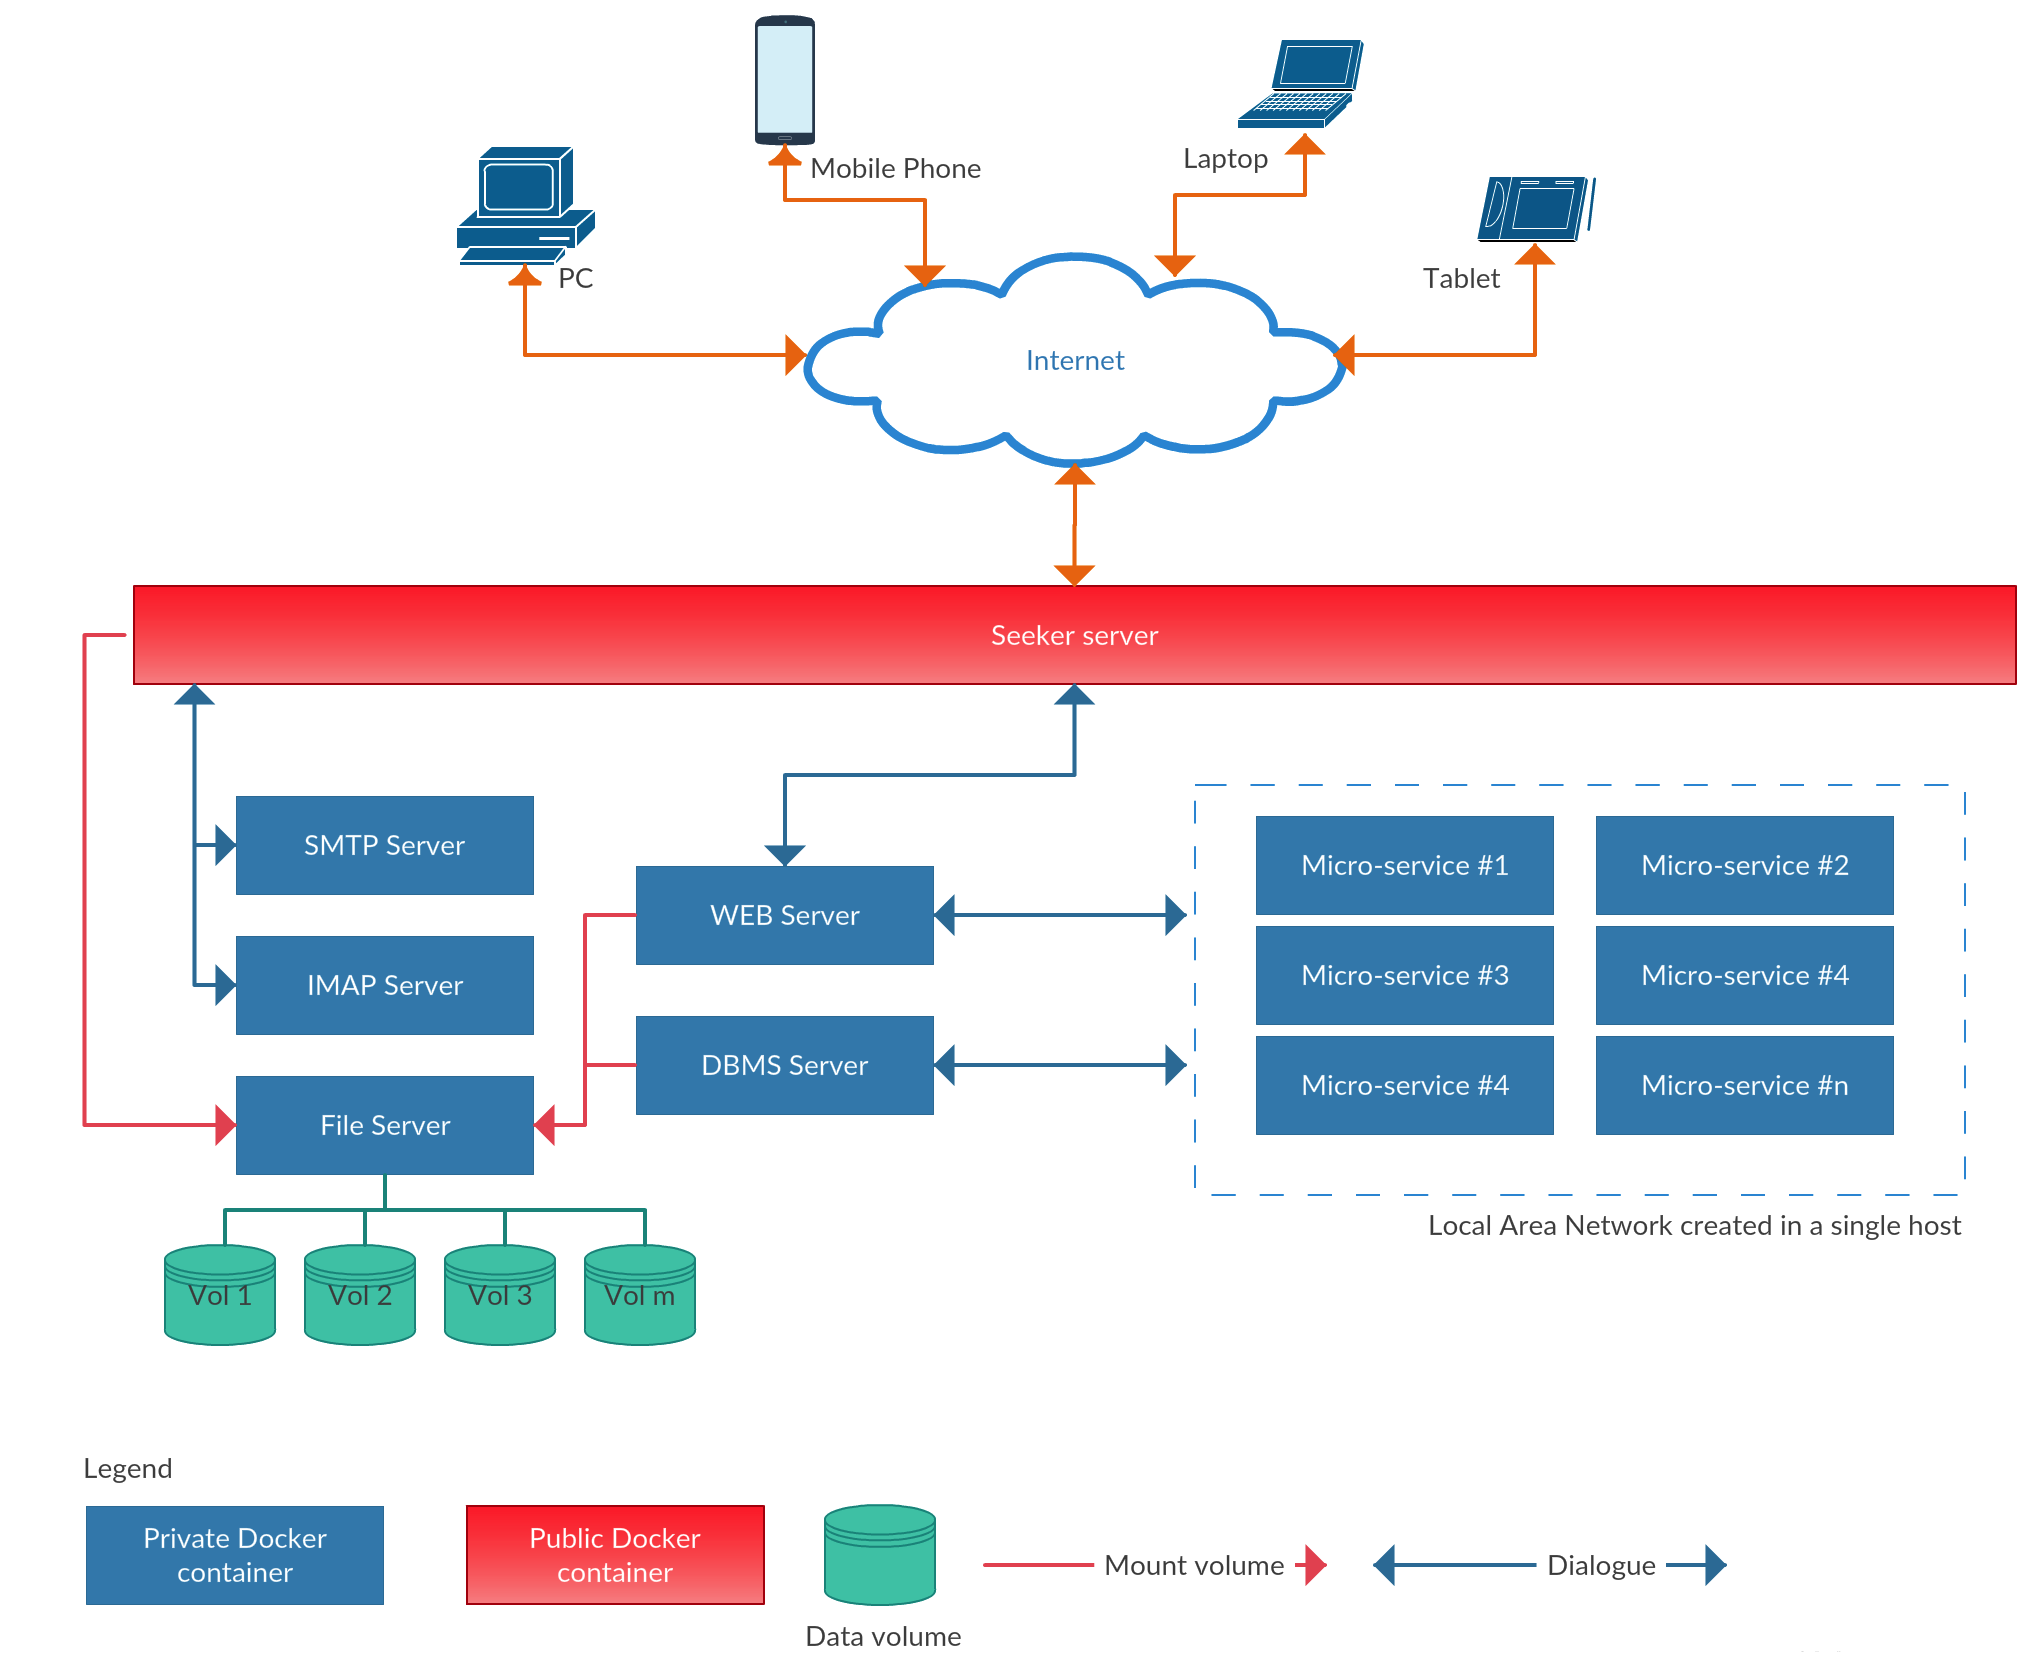
\includegraphics[width=1.2\textwidth, angle=90]{chapters/architecture/images/architecture.png}
	\caption[Proposed architecture]{Overview of a possible elastic and multi-tenant architecture that
		exploits the Docker containers.}
	\label{img:architecture-proposal-architecture}
\end{figure}

As we can see from the diagram, the architecture is composed by two different type of node:

\begin{itemize}
	\item{\keyword{private}: nodes that are only able to communicate with other nodes inside
		the same network;}
	\item{\keyword{public}: it is able to communicate with other nodes inside the same network
		and also accept incoming communications coming from Internet.}
\end{itemize}

A key component of our architecture is the \keyword{seeker server}. This is the key component that will
be able to manage all the elasticity requirements. We call it \keyword{project ``ingress''} and will
describe it in the next Section.

\subsubsection{Ingress project}
\label{sec:architecture-proposal-architecture-ingress}
The main scope of the project is to provide a single and coherent access point, in which it is possible
to check all the incoming connection before they reach the \ac{vpn} network where the micro-services are
deployed.

Its main characteristics are:

\begin{itemize}
	\item{\keyword{security \& authentication}: it have to check, for each connection, all the necessary
		access requirements (loaded from a system database inside the File Server) before tenants are able
		to reach the desired resource;}
	\item{\keyword{monitoring}: it have to able to monitor the incoming traffic in order to correctly bill
		consumed resources to each tenant subscribed to the service;}
	\item{\keyword{dynamic routing}: it have to route each request to the most appropriate micro-service;}
	\item{\keyword{manage workload}: it have to manage the incoming workload in order to scale-in/scale-out
		micro-services only when necessary; it is also able to stop containers that have not incoming connection
		to manage\footnote{It is not convenient stop a container after each connection, but we have to build a
		technique like a ``watchdog''.};}
	\item{\keyword{static cache}: it is able to provide a static cache in order to reduce the latency time
		when clients access to static contents.}
\end{itemize}

This component will encapsulate a properly designed algorithm that on the basis of the actual workload
will be able to scale-in/out the necessary micro-services contained inside the private nodes (see Figure
\ref{img:architecture-proposal-architecture}). This algorithm will be based on the 
``monitor-analyse-plan-execute'' major-cycle described in Section \ref{sec:elasticity-requirements-autonomy}.

Thanks to the increasing inclusion of the Docker \acs{api} inside the modern programming languages, will be
quite easy for this component to manage containers' life-cycle in order to replicate/close them when necessary.
Through managing containers' life-cycle we are able to scale our service and adapt it to current workloads.

Another key point is in having a ``\keyword{filter battery}'' capable to ``\keyword{execute actions}'' on the
incoming requests if pre-determined criteria are satisfied. Figure 
\ref{img:architecture-proposal-architecture-ingress} shows a diagram that illustrate how each incoming request
will be managed before and after it reaches the service.

\begin{figure}
	\centering{}
	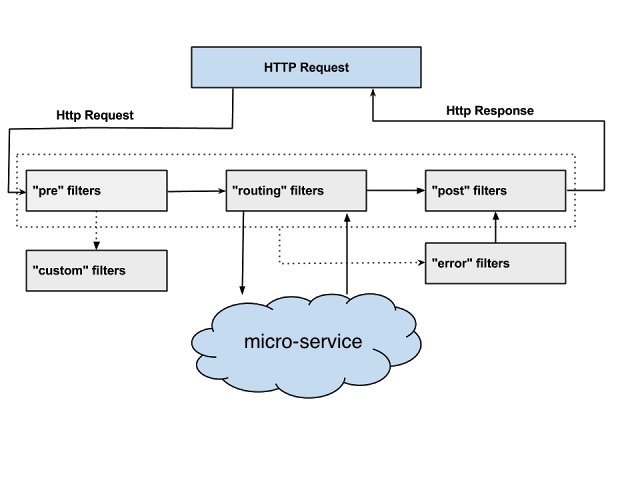
\includegraphics[width=0.8\textwidth]{chapters/architecture/images/ingress-design.png}
	\caption[Request management by ingress]{Algorithm that manage all the incoming requests to our
		services.}
	\label{img:architecture-proposal-architecture-ingress}
\end{figure}

The filter main characteristics are:

\begin{itemize}
	\item{\keyword{filter typlogy}: determine when the filter must be executed; possibility are:}
	\begin{itemize}
		\item{PRE: before the request reaches the micro-service, here we can make necessary security
			and authorization checks;}
		\item{ROUTING: decide to which micro-service route the incoming request, if the preceding
			checks performed successfully;}
		\item{POST: after the request reaches the micro-service, here we are able to format the response
			before send it to the client;}
		\item{ERROR: in case a micro-service respond with an error code.}
	\end{itemize}
	\item{\keyword{order}: determine on which order filter on the same level will be executed;}
	\item{\keyword{criteria}: the criteria that must be satisfied in order to apply the current filter;}
	\item{\keyword{action}: the associated action to the filter, executed only if the criteria results
		satisfied.}
\end{itemize}

As we argued this is the key component where the elasticity mechanisms are placed in order to guarantee
high level of performance and \ac{qos}.

\subsubsection{Micro-service network}
\label{sec:architecture-propoasal-architecture-network}
After having analysed the network costs (see Section \ref{sec:measurements-network-result}) we have
understood that it is necessary to locate containers with micro-services as much as possible inside 
the same physical host in order to reduce latency costs. Thus, we have decided to place the private
containers inside the same host linked together with the ``link'' capabilities provided by Docker
(see Section \ref{sec:background-deployments-docker-architecture}).

Creating a \ac{vpn}, as shown in Figure \ref{img:architecture-proposal-architecture}, with the
micro-services also increases the security performance because the exact network and micro-service
configuration will be hidden to the outside world. To increase further the security performance we must
pay attention in creating connections only with the ``seeker'' node  or with nodes inside the same
\ac{vpn} (avoid connection over Internet as much as possible).

Finally, in order create good entry/exit points in each micro-service we want to adopt, as much as possible,
the \ac{amqp} protocol. This protocol avoid unnecessary synchronization between services allowing them
to serve multiple tenants concurrently.

\subsubsection{Multi-tenancy management}
\label{sec:architecture-propoasal-architecture-multiTenancy}
As we argued in Section \ref{sec:elasticity-multiTenancy} through good elasticity mechanisms developers
are able to provide multi-tenants applications or services to end-users and companies.

Given our decision to adopt the containerization as a base to support our architecture, and having 
understood the concepts illustrated in Section \ref{sec:architecture-soaRevisitation-microServices-requirements},
we focus our attention in building stateless micro-services, which they are easily shareable between
different tenants.

Micro-services have to contain the business logic of our application or service. Business logic is
the same between all tenants because there is not the presence of proprietary or sensible information\footnote{
	The business logic must process some meta-information, contained inside the incoming requests, that permit to
	distinguish different tenants.}. As a consequence there is the need of lower instances to support all tenants
(instead of having one replica of the service or application for each end-user).

The vertical separation, needed to maintain each tenant divided, must be managed in micro-services
which supervise the persistence layer (the ``File Server'' in Figure
\ref{img:architecture-proposal-architecture}). Exists mainly three possible techniques:

\begin{itemize}
	\item{\keyword{different database file}: each tenants access to a proprietary database file. This solution
		allow an easy schema customization and an high data separation that lead tenants to high level of security;}
	\item{\keyword{single database file multiple schemas}: each tenants access to same database file but access
		only to the associated schema; also in this scenario it is possible to easily customize the tenant's schema.
		In this scenario is more complicated restore data after a disaster because in the same file reside data of
		other tenants;}
	\item{\keyword{single database file single schema}: each tenants access to the same database file and schema.
		The tenants' data are separated by code placed inside the tables that compose the schema. This scenario is
		useful when we want lower costs and support an higher number of tenants by sacrificing some security aspects.
		In addiction, also in this case restore tenants' data after a disaster is more complicated because tenants'
		data are mixed together.}
\end{itemize}

As we just argued each one of the above techniques comes with its pro \& cons. The architecture
proposed in Section \ref{sec:architecture-proposal-architecture} can adopt each one of these
techniques. They represents different subscription types that differentiate the offered services.

Finally, to increase the overall performance will be possible to manage the Docker data-volumes
(see Section \ref{sec:background-deployments-docker-dataManagement}) through Flocker \cite{flockerHomepage}.
Flocker, shown in Figure \ref{img:architecture-proposal-architecture-multiTenancy-Flocker} gives to
ops-teams the tools they need to run containerized stateful services (like databases) in production
environments. Unlike a Docker data-volume which is tied to a single server, a Flocker data-volume,
called a dataset, is portable and can be used with any container in your cluster. Flocker manages Docker
containers and data-volumes together. When developers use Flocker to manage their stateful micro-services,
their volumes will follow the containers when they move between different hosts in the cluster.

\begin{figure}[h!]
	\centering{}
	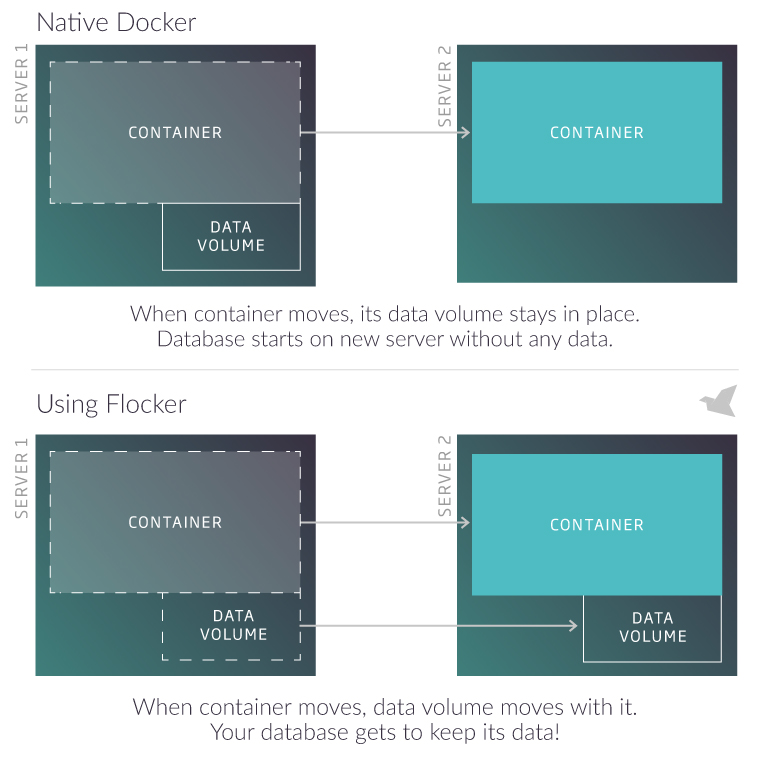
\includegraphics[width=0.6\textwidth]{chapters/architecture/images/flocker.png}
	\caption[Flocker capabilities]{When containers moves, data-volumes moves with it \cite{flockerHomepage}.}
	\label{img:architecture-proposal-architecture-multiTenancy-Flocker}
\end{figure}

\subsection{Related works}
\label{sec:architecture-related}
In literature we have also studied the work done by \citeauthor{baraldo2015reconciling} in
\cite{baraldo2015reconciling}. This is the work done during a preceding Master thesis that also wanted
to analyse the potentiality of the \ac{paas} layer.

The work done in the preceding thesis differs from our because they provide a framework that is able
to deploy an application or a service over differ \ac{iaas} cloud providers. Instead in our proposal
we have to base our service or application inside a \ac{paas} that offers Docker containers, like
Docker data-centre (see Section \ref{sec:background-paas-platforms}).

\begin{figure}
	\centering{}
	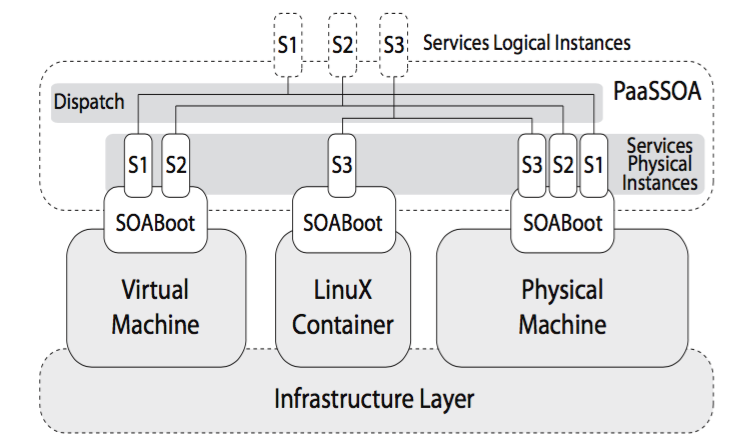
\includegraphics[width=0.6\textwidth]{chapters/architecture/images/passsoa.png}
	\caption[\acs{paas}\acs{soa} framework]{\acs{paas}\acs{soa} framework \cite{baraldo2015reconciling}}
	\label{img:architecture-proposal-related}
\end{figure}

In Figure \ref{img:architecture-proposal-related} we can see a high-level overview of the \ac{paas}\ac{soa}
framework. \ac{soa}Boot agents are responsible for the deploying of a services inside a \ac{iaas} provider,
be it made by \ac{vm}s, containers or physical machines. It create a sort layer that is platform
independent.